\documentclass{handout}

% \SetInstructor{Lt Col James Phillips}
\SetCourseTitle{ECE231: Electrical Circuits and Systems I}
\SetSemester{Spring 2016}
\SetHandoutTitle{Lecture 21: RC and RL Circuit Natural Response}

%\SetDueDate{1 Jan 2016}
%\ShowAllBlanks

\showsoln \setsolncolor{red}

\begin{document}
\maketitle

\textbf{OBJECTIVES:}
\begin{enumerate}
\item .......
\end{enumerate}

\textbf{READING}
\begin{description}
\item [Required]:
\begin{itemize}
\item  Textbook, section 7.1, pages 314--324
\end{itemize}
\item [Optional]: None
\end{description}

\section{A Brief Review of Differential Equations Solution Techniques}
\subsection{Seperation of Variables}
Let's look at the following first order, homogenous differential equation:
\begin{equation}
\frac{\partial v(t)}{\partial t}+\frac{1}{RC}v(t)=0
\end{equation}

We can rewrite this as:
\soln{0.75in}{
\begin{equation}
\frac{1}{v(t)}\partial v(t)=-\frac{1}{RC}\partial t
\end{equation}
where we have seperated the variables, meaning that we have gathered every term that has a v(t) on one side and the other stuff on the other side.
}

Now we integrate both sides:
\soln{2.25in}{
\begin{equation}
\int \frac{1}{v(t)}\partial v(t)=-\int \frac{1}{RC}\partial t
\end{equation}
\begin{equation}
\ln v(t)+ K_1=-\frac{t}{RC} +K_2
\end{equation}
but we can combine our constants
\begin{equation}
\ln v(t)=-\frac{t}{RC} +K
\end{equation}
where $K=K2-K_1$, but really it is just a constant....

Solving for v(t) gives
\begin{equation}
v(t)=e^{-\frac{t}{RC} +K}
\end{equation}
but this simplifies to
\begin{equation}
v(t)=K'e^{-\frac{t}{RC}}
\end{equation}
where $K' = e^K$

The value of $K'$ can be found using initial conditions.
}

\subsection{Undetermined Coefficients}
Let's start with the same differential equation from above:
\begin{equation}
\frac{\partial v(t)}{\partial t}+\frac{1}{RC}v(t)=0
\end{equation}

Any solution to this equation has to be linearly proportional to the derivative of itself.  We can state this mathematically by rearranging the equation:
\soln{0.75in}{
\begin{equation}
\frac{\partial v(t)}{\partial t}=-\frac{1}{RC}v(t)
\end{equation}
}

\textbf{What function do we know that the derivative has the same form as the original function?}  \soln{0.5}{The exponential funtion}

So, let's guess a solution of the form:
\soln{0.75in}{
\begin{equation}
v(t) = Ke^{st}
\end{equation}
}

Now, we can plug that into our original differential equation:
\soln{0.75in}{
\begin{equation}
\frac{\partial Ke^{st}}{\partial t}=-\frac{1}{RC}Ke^{st}
\end{equation}
}

Take the derivative:
\soln{0.75in}{
\begin{equation}
Kse^{st}=-\frac{1}{RC}Ke^{st}
\end{equation}
}

Therefore
\soln{0.75in}{
\begin{equation}
s=-\frac{1}{RC}
\end{equation}
\begin{equation}
v(t)=Ke^{-\frac{t}{RC}}
\end{equation}
Same as before!
}

$K$ is found using initial conditions.  More on that later....

\newpage
\clearpage
\pagebreak

\section{RC \& RL Circuit Analysis}


Let's start by writing the differential equations for a couple of simple circuits:

\textbf{Example 1} -- Write the differential equations for the circuits shown in Figure \ref{fig: Example1}

\begin{figure} [h!]
\centering
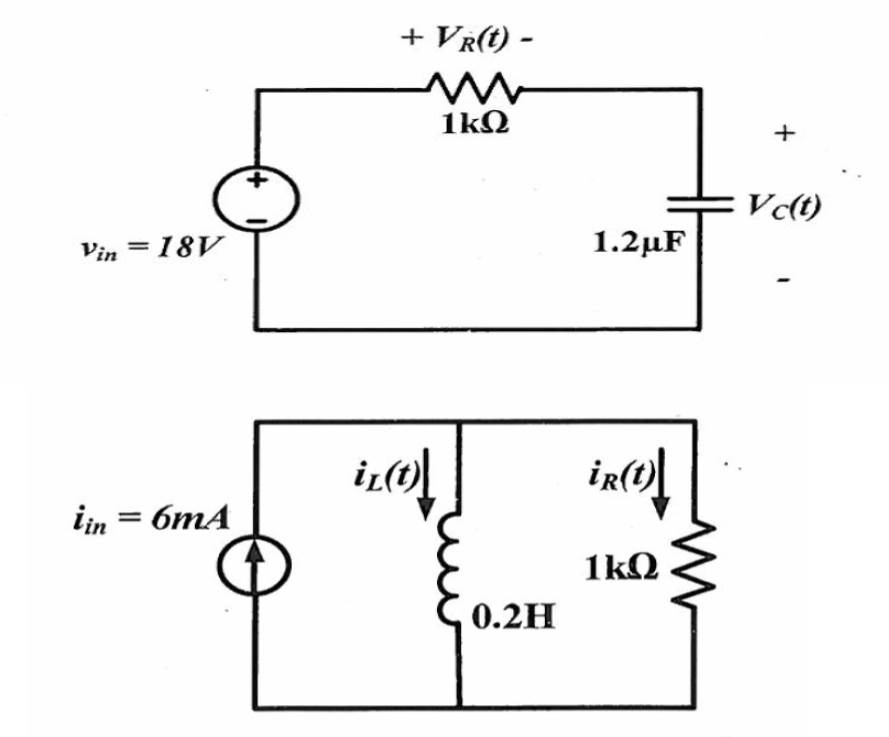
\includegraphics[width=0.5\textwidth]{Example1.jpg}
\caption{Circuits for Example 1}
\label{fig: Example1}
\end{figure}

\soln{4in}{
Circuit \#1
\begin{equation}
v_r(t) + v_c(t) = 18\ V \nonumber
\end{equation}
\begin{equation}
i_r(t)R + v_c(t) = 18\ V \nonumber
\end{equation}
but $i_r(t)=i_c(t)$, therfore
\begin{equation}
i_c(t)R + v_c(t) = 18\ V \nonumber
\end{equation}
\begin{equation}
CR\frac{\partial v_c(t)}{\partial t} + v_c(t) = 18\ V \nonumber
\end{equation}
\begin{equation}
\frac{\partial v_c(t)}{\partial t} +\frac{1}{RC} v_c(t) = \frac{1}{RC}18\ V \nonumber
\end{equation}
Circuit \#2
\begin{equation}
i_L(t)+i_R(t) = 6\ mA
\end{equation}
\begin{equation}
i_L(t)+\frac{v_R(t)}{R} = 6\ mA
\end{equation}
but since $v_R(t) = v_L(t)$
\begin{equation}
i_L(t)+\frac{v_L(t)}{R} = 6\ mA
\end{equation}
\begin{equation}
i_L(t)+\frac{L}{R}\frac{\partial i_L(t)}{\partial t} = 6\ mA
\end{equation}
\begin{equation}
\frac{\partial i_L(t)}{\partial t} + \frac{R}{L}  i_L(t)=\frac{R}{L} 6\ mA
\end{equation}

}

\newpage
\clearpage
\pagebreak

When analyzing RC or RL circuits, the analysis can be broken into three parts:
\soln{2in}{
\begin{enumerate}
\item Steady state ($t<0$), leading up to our initial conditions.  Usually we consider the circuit to have been in this state for a ``long time''
\item Transient Respsonse.  This is the interesting part..... and the part we are most interested in.  This is where the dynamic element (Capacitor or Inductor) has an impact on the circuit
\item Steady state..... After some time our circuit element will return to steady state
\end{enumerate}
}

Additionally, we can look at two types of circuit responses:
\soln{2in}{
\begin{description}
\item[Natural Response] -- This is the response to a homogenous differential equation.  For $t>0$, there are no sources in the circuit; only the initial conditions drive the response.
\item[Forced Response] -- This is the repsonse to a non-homogenous differential equations; this means for $t>0$ there are sources in the circuit.  Typically initial conditions are set to zero when looking at forced response.
\end{description}
}

Today we will look at natural response and will deal with forced responses next lesson.

Let's first look at a simple circuit that shows the time response of a discharging capacitor.  See Figure \ref{fig: DischargingCapacitorCircuit}.

\begin{figure} [h!]
\centering
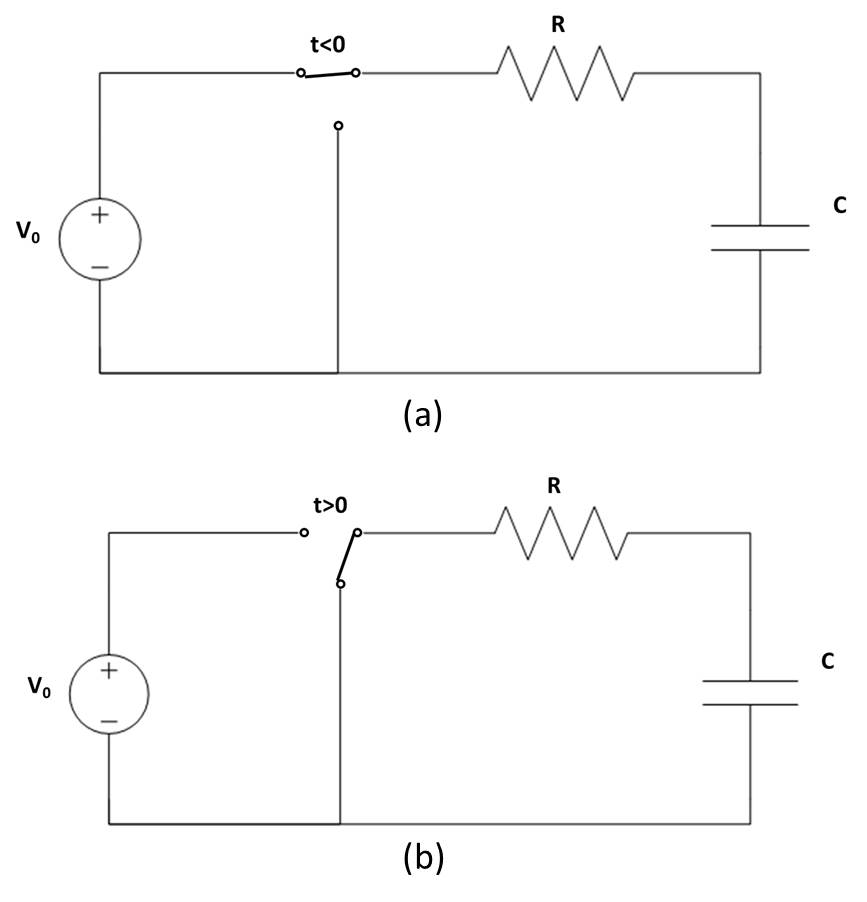
\includegraphics[width=0.5\textwidth]{DischargingCapacitorCircuit.jpg}
\caption{(a) The circuit before the switch is moved (b) the final circuit, after switch is moved}
\label{fig: DischargingCapacitorCircuit}
\end{figure}

Before we move the switch, the voltage across the capacitor eqauls $V_0$; we are assuming the switch has been in this position for a long time (we will talk more about what a long time really means).

At $t=0$ we move the switch and enter the {\em Transient Response} phase of our analysis.  The differential equation for this circuit will look like (this is easily found using KVL):

\begin{equation}
\frac{\partial v_c(t)}{\partial t} +\frac{1}{RC} v_c(t) = 0
\end{equation}

From before we found that the solution to these differential equations have the form:
\begin{equation}
v_c(t)=Ke^{-\frac{t}{RC}}
\end{equation}

To find $K$ we use our initial condition:
\soln{0.5in}{
\[
v_c(0)=V_0
\]
}

which give us:
\soln{0.5in}{
\[
K=V_0
\]
}

So our final circuit response is:
\soln{0.5in}{
\[
v_c(t)=V_0e^{-\frac{t}{RC}}
\]
}

\begin{figure} [h!]
\centering
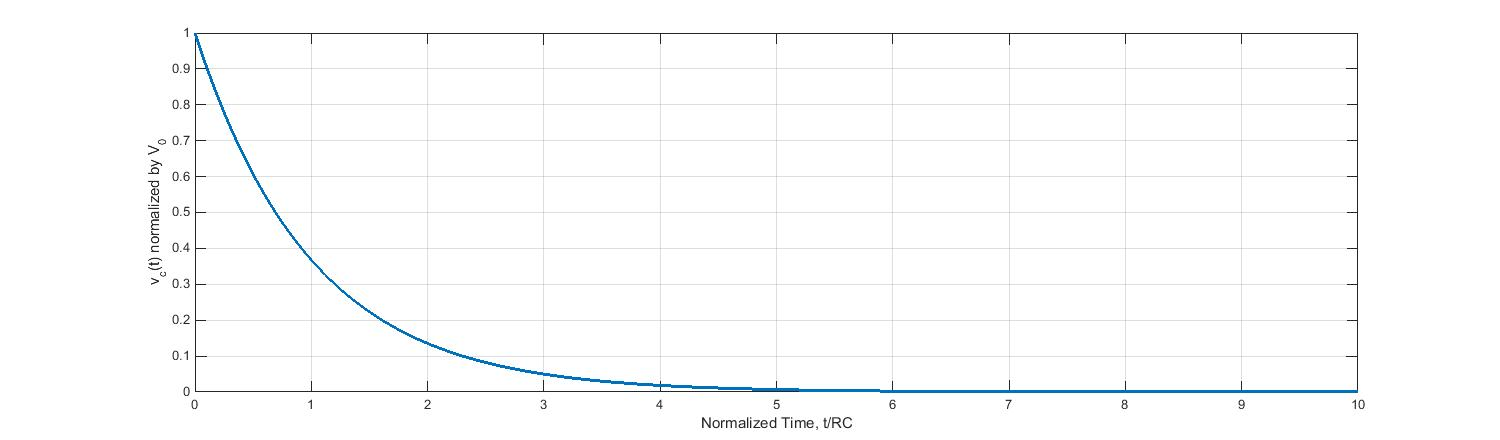
\includegraphics[width=1\textwidth]{CapacitorNaturalResponse.jpg}
\caption{Capacitor Natural Response}
\label{fig: CapacitorNaturalResponse}
\end{figure}

\textbf{What can we learn from this?}

First, we should recognize that this is a decaying exponential function, that starts at $V_0$ and decays to zero.  Second we can see that it is effective zero at time $t=\frac{5}{RC}$.  Recalling from our initial discussion on exponential functions, they go to zero after approximately five time constants.  This leads us to define a time constant, $T_C$ for the $RC$ circuit:
\soln{0.5in}{
\[
T_C = RC
\]
}

So to tie this back to our three analysis phases, we see that for $t<0$, the circuit is in a steady state with a fully charged capacitor.  For $0<t<\frac{5}{RC}$ the circuit is in the transient response phase with the capacitor discharging.  FOr $t>\frac{5}{RC}$ the circuit has returned to a steady state condition.

\newpage
\clearpage
\pagebreak

We can now examine the analagous case for an inductor.  See Figure \ref{fig: DischargingInductorCircuit}.

\begin{figure} [h!]
\centering
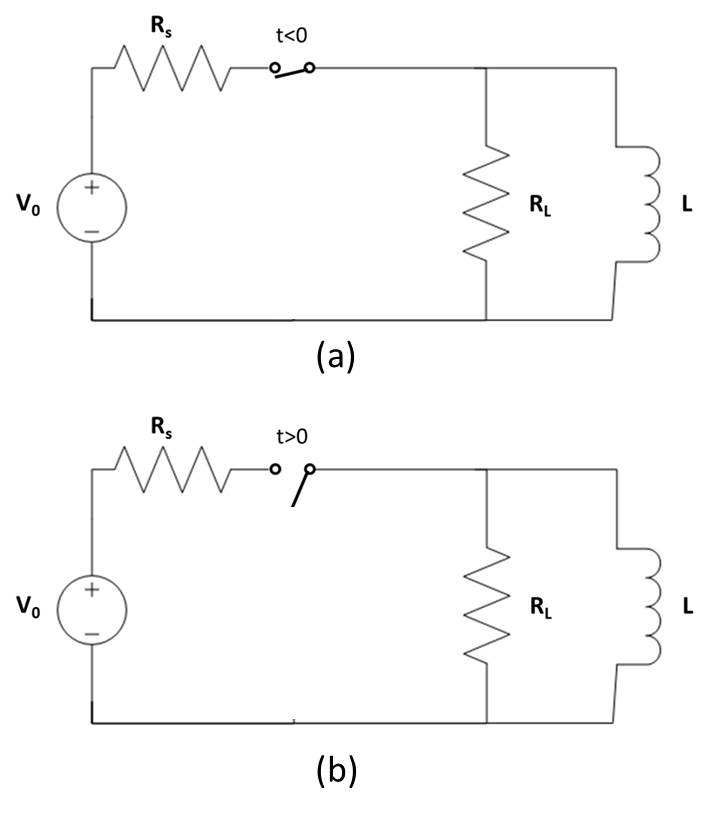
\includegraphics[width=0.5\textwidth]{DischargingInductorCircuit.jpg}
\caption{(a) The circuit before the switch is moved (b) the final circuit, after switch is moved}
\label{fig: DischargingInductorCircuit}
\end{figure}

\textbf{What is the current through the inductor for $t<0$?}

There are a couple of steps or methods to figure this out, but first you have to recall that for steady state D.C. an inductor looks like a short.  This means $R_L$ has no impact on the circuit for $t<0$ since it is shorted out.

Next you simply use Ohm's Law to find the current around the loop (which now effectively contains the voltage source and $R_S$).  This is effectively a source transformation:
\soln{0.5}{
\[
i_L(t\le 0) = \frac{V_0}{R_s}
\]
Later this will serve as our initial condition.
}

The differential equation for $t>0$ is:
\soln{0.5in}{
\[
\frac{\partial i_L(t)}{\partial t} + \frac{R_L}{L}  i_L(t)=0
\]
}

Which one again we know the solution has to have the form:
\soln{0.5in}{
\[
i_L(t) = Ke^{st}
\]
$s$ is just a dummy variable which we can solve for:
\[
\frac{\partial i_L(t)}{\partial t} =- \frac{R_L}{L}  i_L(t)
\]
\[
\frac{\partial Ke^{st}}{\partial t}=Ks^{st} =- \frac{R_L}{L}  Ke^{st}
\]
Therfore
\[
s = -\frac{R_L}{L}
\]
}

Finally $K$ is found using our initial condition:
\soln{0.5}{
\[
K = \frac{V_0}{R_s}
\]

}
So our circuit natrual response is
\soln{0.5}{
\[
i_L(t) = \frac{V_0}{R_s}e^{-\frac{R_L}{L}t}
\]

}
\begin{figure} [h!]
\centering
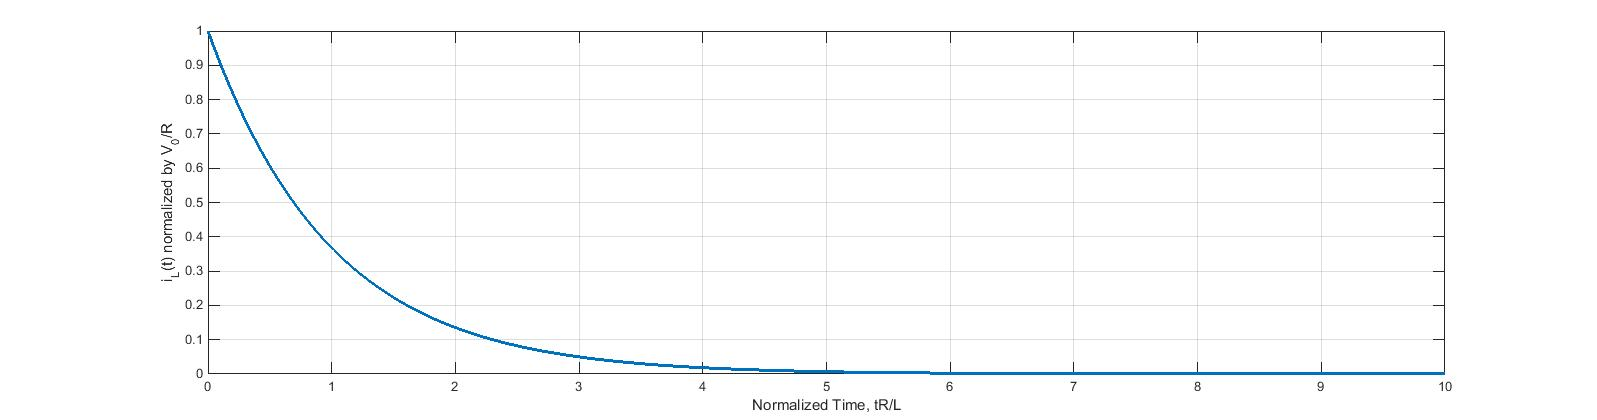
\includegraphics[width=1\textwidth]{InductorNaturalResponse.jpg}
\caption{Inductor Natural Response}
\label{fig: InductorNaturalResponse}
\end{figure}

What you should be able to interpret from this equation and graph is:
\soln{0.5in}{
\[
T_L = \frac{L}{R_L}
\]
}
Where $T_L$ is the time constant for an $RL$ circuit.

Notice this response is the same as the capacitor response (a decaying exponential); the only difference is the capacitor vertical axis is voltage and this inductor vertical axis is current.

\newpage
\clearpage
\pagebreak

\textbf{Example 2} -- For the circuit shown in Figure \ref{fig: Example2}, find $v_c(t)$ and $i(t)$

\begin{figure} [h!]
\centering
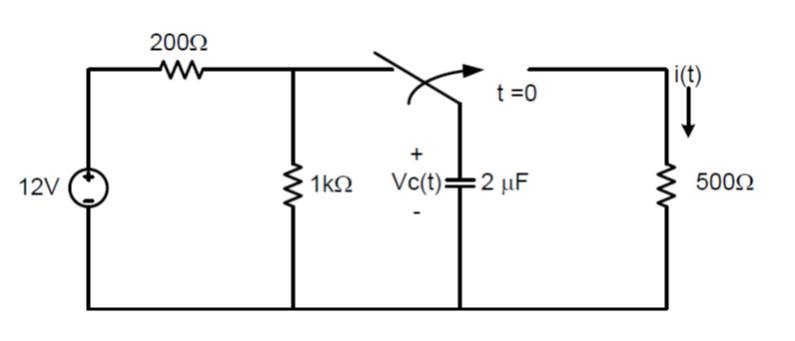
\includegraphics[width=0.75\textwidth]{Example2.jpg}
\caption{Example 2 Circuit}
\label{fig: Example2}
\end{figure}

\soln{6in}{
Assume the switch has been in position 1 long enough for the circuit to reach steady state and find the voltage across the capacitor.  This will be our initial condition, $v_c(0)$.  Since at steady state, a capacitor acts like an open circuit to DC, we can find $v_c(0)$ by a simple voltage divider:
\[
v_c(0) = \frac{1\ k\Omega}{1\ k\Omega+200\ \Omega}12\ V = 10\ V
\]
For $t>0$, the circuit is only the rightmost resistor in a loop with the capacitor.  We can write a KVL equation for that loop:
\[
v_c(t) - v_R(t) = 0
\]
which equals
\[
v_c(t) - i_R(t)R = 0
\]
but we also know that $i_R(t) =-i_c(t)$ (watch signs using passive sign convention) and that
\[
i_c(t) = C\frac{\partial v_c(t)}{\partial t}
\]
which gives
\[
v_c(t) + RC\frac{\partial v_c(t)}{\partial t} = 0
\]
rearraging gives
\[
\frac{\partial v_c(t)}{\partial t}+ \frac{1}{RC}v_c(t) = 0
\]

We know the solution of this differential equation is:
\[
v_c(t)=v_c(0) \times e^{-\frac{1}{RC}t}
\]
plugging in for $v_c(0)=10\ V$, $R=500\ \Omega$ and $C=2\ \mu F$ gives:
\[
v_c(t)=10e^{-1000t}u(t)
\]

Where the $u(t)$ accounts for the fact that this solution is only valid for $t>0$

We can find $i(t)$ by using Ohm's law
\[
i(t) = \frac{v_c(t)}{R} = 20e^{-1000t}u(t)\ mA
\]
you could also have found $i(t)$ by
\[
i_c(t) = C\frac{\partial v_c(t)}{\partial t}
\]
}


\newpage
\clearpage
\pagebreak

\textbf{Example 3} -- For the circuit shown in Figure \ref{fig: Example3}, find $v_c(t)$ and $i(t)$

\begin{figure} [h!]
\centering
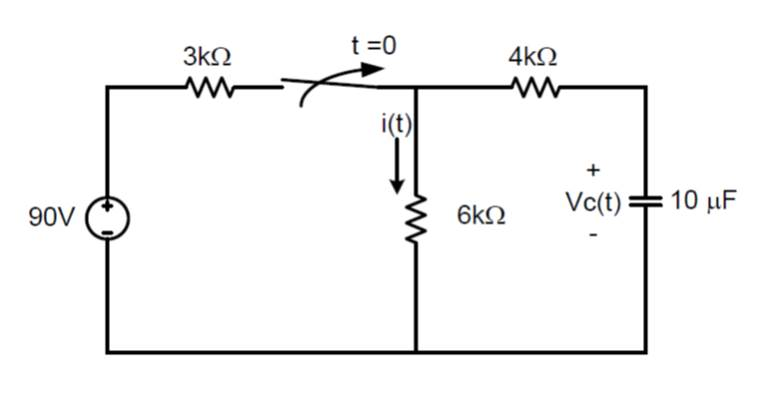
\includegraphics[width=0.75\textwidth]{Example3.jpg}
\caption{Example 3 Circuit}
\label{fig: Example3}
\end{figure}

\soln{6in}{
Like the previous example we can find the initial capacitor voltage, $v_c(0^-)$, by using a voltage divider:
\[
v_c(0) = \frac{6\ k\Omega}{3\ k\Omega+6\ k\Omega}90\ V = 60\ V
\]
Notice the $4\ k\Omega$ resistor had no impact on the initial capacitor voltage since at steady state there is no current through it, therefore, no voltage is dropped across it.

Similar to the last example, when the switch is moved, the new circuit contains no sources, just a capacitance and resistance.  For $t>0$, $R_{eq}=10\ k\Omega$ and $C = 10\ \mu F$.

The differential equation for the circuit is:
\[
\frac{\partial v_c(t)}{\partial t}+ \frac{1}{RC}v_c(t) = 0
\]
and the solution has the form:
\[
v_c(t)=v_c(0) \times e^{-\frac{1}{RC}t}
\]
plugging in for $v_c(0)=60\ V$, $R=10\ k\Omega$ and $C=10\ \mu F$ gives:
\[
v_c(t)=60e^{-10t}u(t)\ V
\]
We can find $i(t)$ by using Ohm's law
\[
i(t) = \frac{v_c(t)}{R} = 6e^{-10t}u(t)\ mA
\]

}

\newpage
\clearpage
\pagebreak

\textbf{Example 4} -- For the circuit shown in Figure \ref{fig: Example4}, find $v_c(t)$ and $i(t)$

\begin{figure} [h!]
\centering
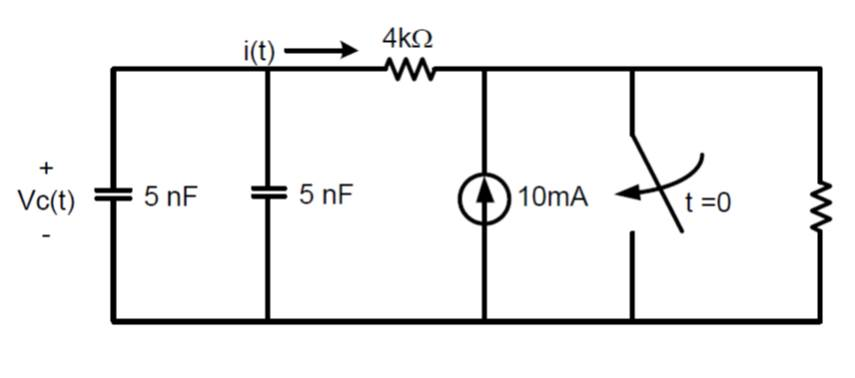
\includegraphics[width=0.75\textwidth]{Example4.jpg}
\caption{Example 4 Circuit}
\label{fig: Example4}
\end{figure}

\soln{6in}{
\begin{figure} [h!]
\centering
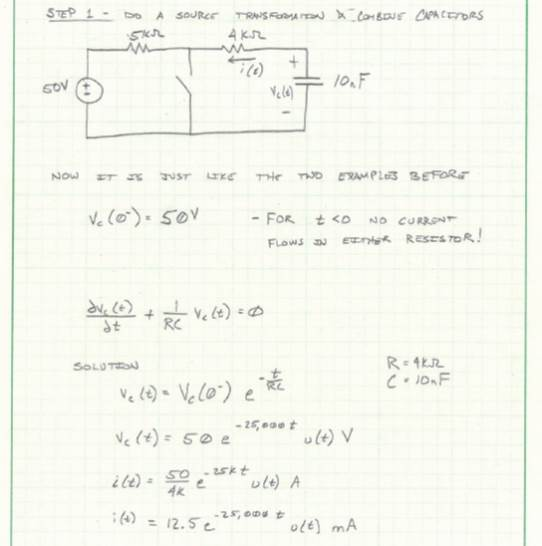
\includegraphics[width=0.9\textwidth]{Example4soln.jpg}
\end{figure}
}



\newpage
\clearpage
\pagebreak

\textbf{Example 5} --For our last example, lets tackle an inductor circuit.....

For the circuit shown in Figure \ref{fig: Example5}, find $i_l(t)$ and $v(t)$
\begin{figure} [h!]
\centering
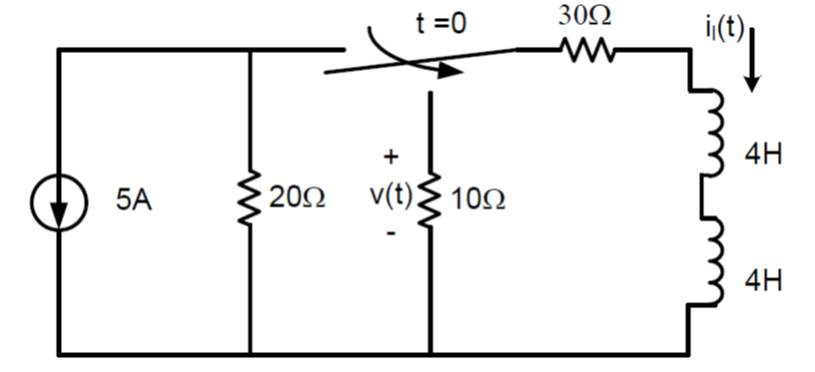
\includegraphics[width=0.5\textwidth]{Example5.jpg}
\caption{Example 5 Circuit}
\label{fig: Example5}
\end{figure}
\soln{6in}{
\begin{figure} [h!]
\centering
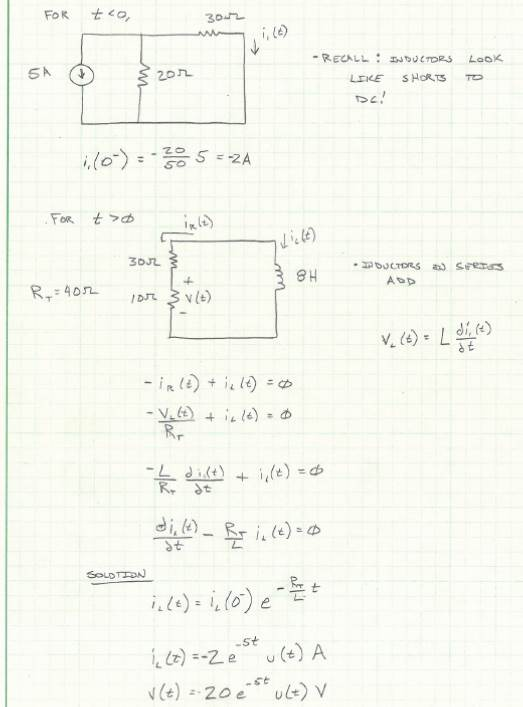
\includegraphics[width=0.7\textwidth]{Example5soln.jpg}
\end{figure}
}
\newpage
\clearpage
\pagebreak

\end{document}


% Equation Array Example Code
%\begin
%{eqnarray}
%P_R &=& i_R^2R \nonumber \\
%P_R &=& (100\ mA)^2 \times 100\ \Omega \nonumber \\
%P_R &=& (100 \times 10^{-3}\ A)^2 \times 100\ \Omega \\
%P_R &=& 10000 \times 10^{-6}\ A^2  \times 100\ \Omega \nonumber \\
%P_R &=& 1\ W  \nonumber
%\end{eqnarray}

% Figure Example Code
%\begin{figure} [h!]
%\centering
%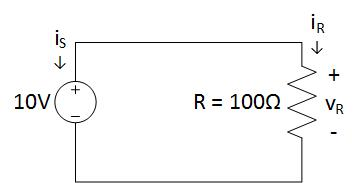
\includegraphics[width=0.5\textwidth]{OhmsLawExampleSolution.jpg}
%\caption{Ohm's Law example circuit}
%\label{fig: OhmsLawExampleSolution}
%\end{figure}

%Table Example Code
%\begin{table}[h]
%\centering
%\begin{tabular}{|l|c|c|}
%\hline
%Prefix & Abbreviation & Value \\
%\hline \hline
%Giga & $G$ & $10^9$ \\
%Mega & $M$ & $10^6$ \\
%Kilo & $k$ & $10^3$ \\
%\hline
%milli & $m$ & $10^{-3}$ \\
%micro & $\mu$ & $10^{-6}$ \\
%nano & $n$ & $10^{-9}$ \\
%pico & $p$ & $10^{-12}$ \\
%\hline
%\end{tabular}
%\caption{Engineering prefixes and values}
%\label{tab: Eng Prefixes}
%\end{table}
